\documentclass[10pt]{article}

\usepackage[margin=0.75in]{geometry}
\usepackage{amsmath,amsthm,amssymb}
\usepackage{xcolor}
\usepackage{cancel}
\usepackage{graphicx}
\usepackage{changepage}
\usepackage{circuitikz}
\usepackage{pgfplots}
\usepackage{physics}
\usepackage{hyperref}
\usepackage{siunitx}
\usepackage{fontspec}
\usepackage{relsize}
\usepackage{subfig}
% \usepackage{sagetex}
\usepackage{minted}
\usepackage{todonotes}
\usepackage{multicol, multirow, booktabs}
\usepackage[breakable]{tcolorbox}
\usepackage[inline]{enumitem}

\theoremstyle{definition}
\newtheorem{problem}{Problem}
\newtheorem{soln}{Solution}

\pgfplotsset{compat=newest}
\usetikzlibrary{lindenmayersystems}
\usetikzlibrary{arrows}
\usetikzlibrary{calc}
\usetikzlibrary{positioning, fit}
\usetikzlibrary{3d, perspective}

\definecolor{incolor}{HTML}{303F9F}
\definecolor{outcolor}{HTML}{D84315}
\definecolor{cellborder}{HTML}{CFCFCF}
\definecolor{cellbackground}{HTML}{F7F7F7}
\newcommand{\ui}{\hat{i}}
\newcommand{\uj}{\hat{j}}
\newcommand{\uk}{\hat{k}}
\newcommand{\ux}{\hat{x}}
\newcommand{\uy}{\hat{y}}
\newcommand{\uz}{\hat{z}}
\newcommand{\primed}[1]{#1^\prime}
\pgfdeclarelayer{background}  
\pgfsetlayers{background,main}
\AtBeginDocument{\RenewCommandCopy\qty\SI}
\newcommand{\justif}[2]{&{#1}&\text{#2}}
\DeclareMathOperator\Arg{Arg}
\DeclareMathOperator{\sgn}{sgn}

\makeatletter
\newcommand{\boxspacing}{\kern\kvtcb@left@rule\kern\kvtcb@boxsep}
\makeatother
\newcommand{\prompt}[4]{
    \ttfamily\llap{{\color{#2}[#3]:\hspace{3pt}#4}}\vspace{-\baselineskip}
}

\newcommand{\thevenin}[2]{
  \begin{center}
    \begin{circuitikz} \draw
      (0,0) -- (2,0) to[battery1, l_=$V_{Th}\eq#1$] (2,2) 
      to[resistor, l_=$R_{Th}\eq#2$] (0,2)
      ;
      \draw [o-] (-.07,2.079);
      \draw [o-] (-.07,0.079);
    \end{circuitikz}
  \end{center}
}

\newcommand{\norton}[2]{
  \begin{center}
    \begin{circuitikz} \draw
      (0,0) -- (3,0) to[american current source, l_=$I_{N}\eq#1$] (3,2) -- (0,2) (2,0)
      to[resistor, l=$R_{N}\eq#2$] (2,2)
      ;
      \draw [o-] (-.07,2.079);
      \draw [o-] (-.07,0.079);
    \end{circuitikz}
  \end{center}
}

\newcommand{\highlight}[1]{\colorbox{yellow}{$\displaystyle #1$}}

\newcommand{\ti}[1]{\widetilde{#1}}

\newfontface{\Kaufmann}{Kaufmann}
\DeclareTextFontCommand{\kf}{\Kaufmann}
\newcommand{\scriptr}{\fontsize{12pt}{12pt}\kf{r}}

\newfontface{\KaufmannB}{Kaufmann Bd BT}
\DeclareTextFontCommand{\kfb}{\KaufmannB}
\newcommand{\bscriptr}{\fontsize{12pt}{12pt}\kfb{r}}

\newcommand{\bv}[1]{\mathbf{#1}}

\title{Math 3150H: Assignment I}
\author{Jeremy Favro (0805980) \\ Trent University, Peterborough, ON, Canada}
\date{\today}

\begin{document}
\maketitle
My student number is 0805980 so $p=9$, $q=5$, and $r=22$.
% PROBLEM 1
\begin{problem}
Consider the second order linear PDE given by
$$pu_{xx}+10pu_{xy}+9pu_{yy}+qu_x+qu_y=8pqx+e^{8ry}$$
\begin{enumerate}[label=(\alph*)]
  \item Find a canonical form of the PDE.
  \item Determine the general solution of the PDE.
  \item Show that the general solution you obtained satisfies the original equation.
\end{enumerate}
\end{problem}
\begin{soln}~
  \begin{enumerate}[label=(\alph*)]
    \item Here we have
          $$\Delta = B^2-4AC=100p^2-4(p)(9p)=64p^2>0$$
          So the PDE is hyperbolic. Now we solve
          $$\frac{dy}{dx}=\frac{B\pm\sqrt{64p^2}}{2A}=\frac{10p\pm8p}{2p}=5\pm4.$$
          Which gives in the plus case
          $$\frac{dy}{dx}=9\implies y=9x+\xi\implies \xi=y-9x$$
          and in the minus case
          $$\frac{dy}{dx}=1\implies y=x+\eta\implies \eta=y-x.$$
          Now we do our partials
          \begin{align*}
             & \xi_x = -9 \qquad \xi_{xx}=0 \qquad \xi_y=1 \qquad \xi_{yy}=0 \qquad \xi_{xy}=0       \\
             & \eta_x = -1 \qquad \eta_{xx}=0 \qquad \eta_y=1 \qquad \eta_{yy}=0 \qquad \eta_{xy}=0.
          \end{align*}
          Now we find our new coefficients. We expect $A_1=C_1=0$ but we'll check just to be sure,
          \begin{align*}
            A_1 & =A\xi_x^2+B\xi_x\xi_y+C\xi_y^2                                     \\
                & =p\cdot(-9)^2+10p\cdot(-9)\cdot(1)+9p\cdot(1)^2                    \\
                & =0                                                                 \\
            B_1 & =2A\xi_x\eta_x+B\left(\xi_x\eta_y+\xi_y\eta_x\right)+2C\xi_y\eta_y \\
                & =2p\cdot(-9)\cdot(-1)+10p\cdot
            \left((-9)\cdot(1)+(1)\cdot(-1)\right)+2\cdot(9p)\cdot(1)\cdot(1)        \\
                & = -64p                                                             \\
            C_1 & =A\eta_x^2+B\eta_x\eta_y+C\eta_y^2                                 \\
                & =p\cdot(-1)^2+10p\cdot(-1)\cdot(1)+9p\cdot(1)^2                    \\
                & =0                                                                 \\
            D_1 & =A\xi_{xx}+B\xi_{xy}+C\xi_{yy}+D\xi_{x}+E\xi_{y}                   \\
                & =q\cdot(-9)+q\cdot(1)                                              \\
                & =-8q                                                               \\
            E_1 & =A\eta_{xx}+B\eta_{xy}+C\eta_{yy}+D\eta_{x}+E\eta_{y}              \\
                & =q\cdot(-1)+q\cdot(1)                                              \\
                & =0                                                                 \\
            F_1 & =0                                                                 \\
            G_1 & =pq\left(\eta-\xi\right)+e^{r\left(9\eta-\xi\right)}
          \end{align*}
          Where for $G_1$ we've made the substitution
          \begin{align*}
            x & =\frac{1}{8}\left(\eta-\xi\right)   \\
            y & =\frac{1}{8}\left(9\eta-\xi\right).
          \end{align*}
          This gives our new canonical form PDE as:
          $$64pu_{\xi\eta}+8qu_\xi=pq\left(\xi-\eta\right)-e^{r\left(9\eta-\xi\right)}$$
    \item First we integrate with respect to $\xi$,
          \begin{align*}
            \int64pu_{\xi\eta}+8qu_\xi\,d\xi & =\int pq\left(\xi-\eta\right)-e^{r\left(9\eta-\xi\right)}\,d\xi                         \\
            64pu_{\eta}+8qu                  & =\frac{e^{9r{\eta} - r{\xi}}}{r} + \frac{pq{\xi} \left({\xi} - 2{\eta}\right)}{2}       \\
            u_{\eta}+\frac{8q}{64p}u         & =\frac{e^{9r{\eta} - r{\xi}}}{64pr} + \frac{pq{\xi} \left({\xi} - 2{\eta}\right)}{128p} \\
          \end{align*}
          Which is a linear first order ODE so we find an integrating factor $\mu$,
          $$\mu=\exp\left(\int\frac{8q}{64p}\,d\eta\right)=\exp\left(\frac{8q}{64p}\eta\right).$$
          This gives us
          \begin{align*}
            u\exp\left(\frac{8q}{64p}\eta\right) & =\int\exp\left(\frac{8q}{64p}\eta\right)
            \left[\frac{e^{9r{\eta} - r{\xi}}}{64pr} + \frac{pq{\xi} \left({\xi} - 2{\eta}\right)}{128p}\right]\,d\eta                                                                                                                                                         \\
                                                 & =\frac{\left(2qe^{9r{\eta}} - 2pqr \left(72pr + q\right) {\xi}e^{r{\xi}} {\eta} + pr \left(72pr + q\right) {\xi} \left(q{\xi} + 16p\right) e^{r{\xi}}\right) e^{\frac{q{\eta} - 8pr{\xi}}{8p}}}{16qr \left(72pr + q\right)}
          \end{align*}
          Transforming this back to something in terms of $x$ and $y$ we get
          \begin{align*}
            u & =\exp\left(-\frac{8q}{64p}(y-x)\right)\frac{2qe^{9r{(y-x)}} - 2pqr \left(72pr + q\right) {(y-9x)}e^{r{(y-9x)}} {(y-x)} + pr \left(72pr + q\right) {(y-9x)}\dots}{16qr \left(72pr + q\right)} \\
          \end{align*}
          (Sage used for substitutions).
    \item For this Sage was used to calculate the partials and simplify the expression.
          \begin{tcolorbox}[breakable, size=fbox, boxrule=1pt, pad at break*=1mm,colback=cellbackground, colframe=cellborder]
            \prompt{In}{incolor}{1}{\boxspacing}
            \begin{minted}[breaklines, autogobble]{sage}
x,y,p,q,r = var("x y p q r")

f = ((2 * q * e^(9 * r * (y - x)) + p * r * (72 * p * r + q) * (y - 9 * x) * (q * (y - 9 * x) + 16 * p) * e^(r * (y - 9 * x)) - 2 * p * q * r * (72 * p * r + q) * (y - 9 * x) * (y - x) * e^(r * (y - 9 * x))) * e^((q * (y - x) - 8 * p * r * (y - 9 * x)) / (8 * p) - (q * (y - x)) / (8 * p))) / (16 * q * r * (72 * p * r + q))

ux = diff(f, x)
uxx = diff(ux, x)
uy = diff(f, y)
uyy = diff(uy, y)
uxy = diff(ux, y)

PDE = p*uxx+ 10*p*uxy+9*p*uyy+q*ux+q*uy 
show(PDE.full_simplify())
              \end{minted}
          \end{tcolorbox}
          \begin{tcolorbox}[breakable, size=fbox, boxrule=.5pt, pad at break*=1mm, opacityfill=0]
            \prompt{Out}{outcolor}{1}{\boxspacing}
            $\displaystyle 8 p q x + e^{\left(8 r y\right)}$
          \end{tcolorbox}
  \end{enumerate}
\end{soln}

% PROBLEM 2
\begin{problem}
Use the method of characteristics to solve the IVP
$$u_y+R(x,y)u_x=ru;\qquad u(x,0)=x^r,\quad R(x,y)=\left(1-x\right)\left(p-q\sin\left(qy\right)\right)-p\left(1-x\right)^2e^{py}\sin\left(qy\right)$$
\end{problem}
\begin{soln}
  From the IVP we obtain
  \begin{align*}
             & \frac{dx}{dt}=R(x,y); \qquad \frac{dy}{dt}=1; \qquad \frac{dz}{dt}=r \\
    \implies & \qquad y=t+C_2\implies y=t; \qquad z=rt+C_3.
  \end{align*}
  Now we need to solve
  $$\frac{dx}{dt}=R(x,t)=\left(1-x\right)\left(p-q\sin\left(qt\right)\right)-p\left(1-x\right)^2e^{pt}\sin\left(qt\right)$$
  before we can move on.
  If we make the substitution
  $$k=1-x\implies dk=-dx$$
  we obtain
  $$-\frac{dk}{dt}=k\left(p-q\sin\left(qt\right)\right)-pk^2e^{pt}\sin\left(qt\right)$$
  which we rearrange to
  $$\frac{dk}{dt}+k\left(p-q\sin\left(qt\right)\right)=pk^2e^{pt}\sin\left(qt\right).$$
  This is a Bernoulli equation. So we divide through by $k^2$,
  $$k^{-2}\frac{dk}{dt}+k^{-1}\left(p-q\sin\left(qt\right)\right)=pe^{pt}\sin\left(qt\right)$$
  and we'll let $v=k^{-1}\implies dv = -k^{-2}dt$ which gives
  $$-\frac{dv}{dt}+v\left(p-q\sin\left(qt\right)\right)=pe^{pt}\sin\left(qt\right).$$
  We rearrange this to
  $$\frac{dv}{dt}+v\left(q\sin\left(qt\right)-p\right)=-pe^{pt}\sin\left(qt\right).$$
  We now apply an integrating factor
  $$\mu=\exp\left(\int \left(q\sin\left(qt\right)-p\right)dt\right)=C\exp\left(-\cos(qt)-pt\right)$$
  which gives
  $$\exp\left(-\cos(qt)-pt\right)dv+\left(\exp\left(-\cos(qt)-pt\right)\left(q\sin (qt)-p\right)v+\frac{p\sin(qt)}{\exp(\cos(qt))}\right)dt=0.$$
  This is an exact equation.
  We have
  $$M=\exp\left(-\cos(qt)-pt\right)$$
  and
  $$N=\exp\left(-\cos(qt)-pt\right)\left(q\sin (qt)-p\right)v+\frac{p\sin(qt)}{\exp(\cos(qt))}.$$
  So we look for some $F(v,t)$ such that
  $$dF=Mdv+Ndt$$
  and
  $$\frac{\partial F}{\partial v}=M;\quad \frac{\partial F}{\partial t}= N.$$
  These are both easily solved by direct integration,
  \begin{align*}
    F & =\int \exp\left(-\cos(qt)-pt\right)\left(q\sin (qt)-p\right)v+\frac{p\sin(qt)}{\exp(\cos(qt))}\,dt\\
      & =\frac{p}{q}e^{-\cos qt}+ve^{-\cos (qt)-pt}+C(v).
  \end{align*}
  Differentiating this now with respect to $v$ and setting equal to $M$ we get
  $$
    \frac{\partial F}{\partial v} = e^{-\cos (qt)-pt}+\primed{C}(v)=\exp\left(-\cos(qt)-pt\right)\implies \primed{C}(v)=0.
  $$
  So our solution is 
  $$
  F(t,v)=\frac{p}{q}e^{-\cos qt}+ve^{-\cos (qt)-pt}=C\implies v=Ce^{\cos(qt)+pt}-\frac{p}{q}e^{pt}.
  $$
  Now we back substitute for $v=k^{-1}$,
  $$k^{-1}=Ce^{\cos(qt)+pt}-\frac{p}{q}e^{pt}$$
  and then back substitute for $k=1-x$,
  $$x = \frac{q}{Ce^{\cos(qt)+pt}+pe^{pt}}+1.$$
  Now using our initial condition we can say that
  $$x(0)=\frac{q}{C_1e^{\cos(0)+p\cdot(0)}+pe^{0}}+1=\frac{q}{C_1e+p}+1=s\implies C_1 = \left(\frac{q}{s-1}-p\right)e^{-1}.$$
  Now our initial condition on $z$,
  $$z(0)=C_3=s^r\implies z=rt+s^r.$$
  So we have
  $$x=\frac{q}{ \left(\frac{q}{s-1}-p\right)e^{\cos(qt)+pt-1}+pe^{pt}}+1;\qquad y=t;\qquad z=rt+s^r.$$
  Solving the $x$ expression for $s$ (and substituting $t=y$) we get that 
  $$s = \frac{{\left(p + q\right)} e^{\left(p y + \cos\left(q y\right) - 1\right)} - p e^{\left(p y\right)} - q}{p e^{\left(p y + \cos\left(q y\right) - 1\right)} - p e^{\left(p y\right)} - q}
  \implies z = ry+\left[\frac{q e^{\left(p y + \cos\left(q y\right) - 1\right)}}{p e^{\left(p y + \cos\left(q y\right) - 1\right)} - p e^{\left(p y\right)} - q}\right]^r
  $$
  Which isn't actually a solution so obviously I've gone wrong somewhere. 
\end{soln}

% PROBLEM 3
\begin{problem}
Use SAGE or otherwise to show that a transformation of a second order linear PDE to its canonical form does not alter the classification of the PDE.
\end{problem}
\begin{soln}
  Given that for the PDE
  $$Au_{xx}+Bu_{xy}+Cu_{yy}+Du_x+Eu_y+Fu=G$$
  has discriminant
  $$\Delta=B^2-4AC$$
  and can be transformed into a canonical form with (disregarding other terms as they do not affect $\Delta$)
  \begin{align*}
    A_1 & =A\xi_x^2+B\xi_x\xi_y+C\xi_y^2                                     \\
    B_1 & =2A\xi_x\eta_x+B\left(\xi_x\eta_y+\xi_y\eta_x\right)+2C\xi_y\eta_y \\
    C_1 & =A\eta_x^2+B\eta_x\eta_y+C\eta_y^2.
  \end{align*}
  we can say that the discriminant of the new PDE in the $(\xi,\eta)$ plane will be
  \begin{align*}
    \Delta_1 & = B_1^2-4A_1C_1                                                                                                                                                                                                         \\
             & = B_1^2-4A_1C_1                                                                                                                                                                                                         \\
             & = (2A\xi_x\eta_x+B\left(\xi_x\eta_y+\xi_y\eta_x\right)+2C\xi_y\eta_y)^2-4(A\xi_x^2+B\xi_x\xi_y+C\xi_y^2)(A\eta_x^2+B\eta_x\eta_y+C\eta_y^2)                                                                             \\
             & = \left(B^{2} - 4 A C\right) \eta_{y}^{2} \xi_{x}^{2} - 2 {\left(B^{2} - 4 A C\right)} \eta_{x} \eta_{y} \xi_{x} \xi_{y} + {\left(B^{2} - 4 A C\right)} \eta_{x}^{2} \xi_{y}^{2}\justif{\quad}{Sage's full\_simplify()} \\
             & = \left(B^{2} - 4 A C\right)\left(\eta_{y} \xi_{x}-\eta_{x} \xi_{y}\right)
  \end{align*}
  which we can see is
  $$J^2\Delta.$$
  Because we started with canonical forms by making a change of variables with non-singular (real) Jacobian
  $$
    J=\begin{vmatrix}
      \xi_x  & \xi_y  \\
      \eta_x & \eta_y
    \end{vmatrix}\implies \sgn J^2\Delta = \sgn \Delta
  $$
  which will return the same classification as we originally had in the $x,y$ plane.
\end{soln}

% PROBLEM 4
\begin{problem}
Consider the functions
\begin{align*}
  f_1(x) & =\begin{cases}
              r,       & -p<x<0 \\
              e^{-qx}, & 0<x<p
            \end{cases} \\
  f(x)=e^{-qx},\quad 0<x<p
\end{align*}
\begin{enumerate}[label=(\alph*)]
  \item Find the Fourier sine series of $f_1(x)$
  \item Find the Fourier sine series of $f(x)$ on $\left[0,p\right]$
  \item Find the Fourier cosine series of $f(x)$ on $\left[0,p\right]$
  \item Sketch the appropriate periodic extensions of the functions for each of the above series.
  \item Sketch the graph of each of the above series.
\end{enumerate}
\end{problem}
\begin{soln}
  \begin{enumerate}[label=(\alph*)]
    \item Our coefficient here is
          \begin{align*}
            b_n & = \frac{1}{p}\left[\int_{-p}^{p}f_1(x)\sin\left(n\pi x/p\right)\,dx\right]                                                                              \\
                & = \frac{1}{p}\left[\int_{-p}^{0}r\sin\left(n\pi x/p\right)\,dx
            +\int_{0}^{p}e^{-qx}\sin\left(n\pi x/p\right)\,dx\right]                                                                                                      \\
                & = \frac{1}{p}\left[\eval{-\frac{pr}{n\pi}\cos\left(n\pi x/p\right)}_{-p}^{0}
            -\eval{\frac{1}{q^{2} + (n\pi/p)^2}e^{-qx} \left(q \sin\left(\frac{n\pi x}{p}\right) + \frac{n\pi}{p}\cos\left(\frac{n\pi x}{p}\right)\right)}_{0}^{p}\right] \\
                & = \frac{1}{p}\left[
              \frac{pr}{n\pi}\left[-\cos\left(0\right)
                +\cos\left(-n\pi\right)\right]
              +
              \frac{1}{q^{2} + (n\pi/p)^2}\left[
                e^{-qp} \left(q \sin\left(n\pi\right) + \frac{n\pi}{p}\cos\left(n\pi\right)\right)
                -\left(q \sin\left(0\right) + \frac{n\pi}{p}\cos\left(0\right)\right)
            \right]\right]                                                                                                                                                \\
                & = -\left[
            \frac{r}{n\pi}\left[1
              +(-1)^{n-1}\right]
            +
            \frac{n\pi}{(pq)^2 + (n\pi/p)^2}\left[
            (-1)^{n-1}e^{-qp}+1
            \right]\right]                                                                                                                                                \\
          \end{align*}
          which gives a corresponding Fourier sine series of
          $$\sum_{n=1}^{\infty}-\left[
            \frac{r}{n\pi}\left[1
              +(-1)^{n-1}\right]
            +
            \frac{n\pi}{(pq)^2 + (n\pi/p)^2}\left[
            (-1)^{n-1}e^{-qp}+1
            \right]\right]\sin \left(n\pi x/p\right)$$
    \item Here we have almost the same integral as previously,
          \begin{align*}
            b_n & = \frac{2}{p}\int_{0}^{p}e^{-qx}\sin\left(n\pi x/p\right)\,dx                            \\
                & = \frac{2e^{-pq} \left(n\pi e^{pq} + n\pi\left(-1\right)^{n+1}\right)}{(pq)^2+ (n\pi)^2} \\
          \end{align*}
          which gives a corresponding series of
          $$
            \sum_{n=1}^{\infty}\frac{2e^{-pq} \left(n\pi e^{pq} + n\pi\left(-1\right)^{n+1}\right)}{(pq)^2+ (n\pi)^2} \sin\left(n\pi x/p\right)
          $$
    \item ~
          $$
            a_0=\frac{1}{p}\int_{0}^{p}r\,dx=r
          $$
          and
          \begin{align*}
            a_n & =\frac{2}{p}\int_{0}^{p}e^{-qx}\cos\left(n\pi x/p\right)\,dx                  \\
                & =\frac{2pq\mathrm{e}^{-pq} \left(e^{pq} +(-1)^{n+1}\right)}{(pq)^2+ (n\pi)^2}
          \end{align*}
          which gives a corresponding series of
          $$
            r+\sum_{n=1}^{\infty}\frac{2pq\mathrm{e}^{-pq} \left(e^{pq} +(-1)^{n+1}\right)}{(pq)^2+ (n\pi)^2}\cos\left(n\pi x/p\right)
          $$
    \item ~\begin{center}
            \begin{tikzpicture}
              \begin{axis}[title = {$f_1$},
                  ymax = 25,
                  ymin = -25,
                  xmin=-3,
                  xmax=3,
                  xtick pos = bottom,
                  ytick pos = left,
                  height=0.25\textwidth,
                  width=0.65\textwidth,
                  scale only axis=true,
                  xlabel=$p$,
                  legend pos=north east
                ]
                \draw[red, thick, domain=-3:-2, samples=2] plot (\x, {
                    -22
                  });
                \draw[red, thick, domain=-2:-1, samples=100] plot (\x, {
                    -e^(-5*(\x+2))
                  });
                \draw[red, thick, domain=-1:0, samples=2] plot (\x, {
                    22
                  });
                \draw[red, thick, domain=0:1, samples=100] plot (\x, {
                    e^(-5*\x)
                  });
                \draw[red, thick, domain=1:2, samples=2] plot (\x, {
                    -22
                  });
                \draw[red, thick, domain=2:3, samples=100] plot (\x, {
                    -e^(-5*(\x-2))
                  });
              \end{axis}
            \end{tikzpicture}
            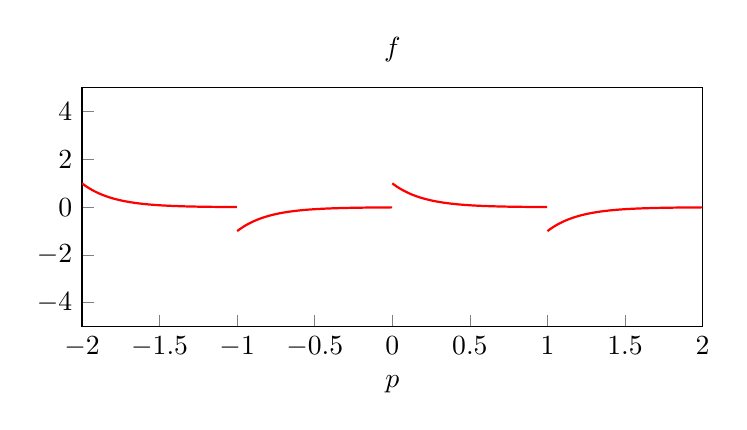
\begin{tikzpicture}
              \begin{axis}[title = {$f$},
                  ymax = 5,
                  ymin = -5,
                  xmin=-2,
                  xmax=2,
                  xtick pos = bottom,
                  ytick pos = left,
                  height=0.25\textwidth,
                  width=0.65\textwidth,
                  scale only axis=true,
                  xlabel=$p$,
                  legend pos=north east
                ]
                \draw[red, thick, domain=-2:-1, samples=100] plot (\x, {
                    e^(-5*(\x+2))
                  });
                \draw[red, thick, domain=-1:0, samples=100] plot (\x, {
                    -e^(-5*(\x+1))
                  });
                \draw[red, thick, domain=0:1, samples=100] plot (\x, {
                    e^(-5*\x)
                  });
                \draw[red, thick, domain=1:2, samples=100] plot (\x, {
                    -e^(-5*(\x-1))
                  });
              \end{axis}
            \end{tikzpicture}
          \end{center}
    \item Sketch the graph of each of the above series.
  \end{enumerate}
\end{soln}

% PROBLEM 5
\begin{problem}
Consider the function
$$
  f(x)=\left(px/r\right)^2+q
$$
defined on $\left[0,r\right]$.

\begin{enumerate}[label=(\alph*)]
  \item Use SageMath to compute the $N^{th}$ partial sum of the Fourier sine series of $f(x)$
        for $N=5,10,50,100$. Plot the partial sums along with the odd extension of $f(x)$
        on the extension interval $\left[-r,r\right]$.
  \item Use SageMath to compute the $N^{th}$ partial sum of the Fourier cosine series of $f(x)$
        for $N=5,10,50,100$. Plot the partial sums along with the odd extension of $f(x)$
        on the extension interval $\left[-r,r\right]$.
  \item Demonstrate the Gibbs Phenomenon from your results.
\end{enumerate}
\end{problem}
\begin{soln}
  \begin{enumerate}[label=(\alph*)]
    \item ~\begin{tcolorbox}[breakable, size=fbox, boxrule=1pt, pad at break*=1mm,colback=cellbackground, colframe=cellborder]
            \prompt{In}{incolor}{1}{\boxspacing}
            \begin{minted}[breaklines, autogobble]{sage}
# Q5 a
clear_vars()
q = 5
p = 9
r = 22
n, x = var('n x')

f = ((p*x/r)^2)+q
# plot function s dashed line to see convergence
f_ext = piecewise([((-r, 0), -f), ((0,r), f)])
func_sin = plot(f_ext, (x, -r, r), color='black', linestyle='dashed')
N = [5, 10, 50, 100] #list of N values to plot over
approx_sin = [] #initialize array of plots
L = r #Define length

b(n) = (2/L) * (integral((f*sin(n*pi*x/L)), x, 0, L))
for i in range (len(N)):
    g(x) = sum((b(n)*sin(n*pi*x/L)) for n in (1..(N[i]+1)))
    approx_sin += [plot(g, (x, -r, r))] #compute and load up plots into array


for i in range (len(N)):
    print("{}th partial sum of Fourier Sine series".format(N[i]))
    gibbs_upper = plot(f(x=r) *1.18, (x, -r, r), color="red") 
    gibbs_lower = plot(-f(x=r) *1.18, (x, -r, r), color="red")
    show(approx_sin[i] + func_sin + gibbs_upper + gibbs_lower) #print out plots with labels
              \end{minted}
          \end{tcolorbox}
          \begin{tcolorbox}[breakable, size=fbox, boxrule=.5pt, pad at break*=1mm, opacityfill=0]
            \prompt{Out}{outcolor}{1}{\boxspacing}
            5th partial sum of Fourier Sine series\\
            \includegraphics[scale=0.75]{graphs/g1s.png}\\
            10th partial sum of Fourier Sine series\\
            \includegraphics[scale=0.75]{graphs/g2s.png}\\
            50th partial sum of Fourier Sine series\\
            \includegraphics[scale=0.75]{graphs/g3s.png}\\
            100th partial sum of Fourier Sine series\\
            \includegraphics[scale=0.75]{graphs/g4s.png}
          \end{tcolorbox}
    \item \begin{tcolorbox}[breakable, size=fbox, boxrule=1pt, pad at break*=1mm,colback=cellbackground, colframe=cellborder]
            \prompt{In}{incolor}{1}{\boxspacing}
            \begin{minted}[breaklines, autogobble]{sage}
# Q5 b
clear_vars()
q = 5
p = 9
r = 22
n, x = var('n x')

f = ((p*x/r)^2)+q
# plot function s dashed line to see convergence
f_ext = piecewise([((-r, 0), f), ((0,r), f)])
func_sin = plot(f_ext, (x, -r, r), color='black', linestyle='dashed')
N = [5, 10, 50, 100] #list of N values to plot over
approx_sin = [] #initialize array of plots
L = r #Define length
a_0 = (1/L) * (integral(f, x, 0, L))
a(n) = (2/L) * (integral((f*cos(n*pi*x/L)), x, 0, L))
for i in range (len(N)):
    g(x) = a_0 + sum((a(n)*cos(n*pi*x/L)) for n in (1..(N[i]+1)))
    approx_sin += [plot(g, (x, -r, r))] #compute and load up plots into array


for i in range (len(N)):
    print("{}th partial sum of Fourier Cosine series".format(N[i]))
    show(approx_sin[i] + func_sin) #print out plots with labels
              \end{minted}
          \end{tcolorbox}
          \begin{tcolorbox}[breakable, size=fbox, boxrule=.5pt, pad at break*=1mm, opacityfill=0]
            \prompt{Out}{outcolor}{1}{\boxspacing}
            5th partial sum of Fourier Cosine series\\
            \includegraphics[scale=0.75]{graphs/g1c.png}\\
            10th partial sum of Fourier Cosine series\\
            \includegraphics[scale=0.75]{graphs/g2c.png}\\
            50th partial sum of Fourier Cosine series\\
            \includegraphics[scale=0.75]{graphs/g3c.png}\\
            100th partial sum of Fourier Cosine series\\
            \includegraphics[scale=0.75]{graphs/g4c.png}
          \end{tcolorbox}
    \item See the red line in the sine series plots. Note that the multiplication by $1.18$ to obtain
          the approximate $9\%$ Gibbs Phenomenon value originates from the expression for $9\%$ of the jump height,
          $$\frac{f(x_j^+)+f(x_j^-)}{2}\cdot0.09=2f(x_j)\cdot0.09=0.18\cdot f(x).$$
  \end{enumerate}
\end{soln}

% PROBLEM 6
\begin{problem}
Recall that an odd function $f(x)$ which is defined on an interval $\left[-L,L\right]$ has a Fourier
series comprised only of sines. Determine an additional symmetric condition on $f(x)$ that will make
the sine coefficients with even indices vanish.
\end{problem}
\begin{soln}
  If $f(x)$ is odd then, as stated in the problem, our Fourier series drops down to
  $$f(x)=\sum_{n=1}^{\infty} b_n\sin\left(n\pi x/L\right)$$
  with
  \begin{align*}
    b_n & =\frac{1}{L}\int_{-L}^{L}f(x)\sin\left(n\pi x/L\right)\,dx                                                                                                       \\
        & =\frac{1}{L}\left(\int_{-L}^{0}f(x)\sin\left(n\pi x/L\right)\,dx+\int_{0}^{L}f(x)\sin\left(n\pi x/L\right)\,dx\right)                                            \\
        & =\frac{1}{L}\left(\int_{0}^{L}f(x)\sin\left(n\pi x/L\right)\,dx+\int_{0}^{L}f(x)\sin\left(n\pi x/L\right)\,dx\right)\justif{\quad}{$x=-x$ in the first integral} \\
        & =\frac{2}{L}\int_{0}^{L}f(x)\sin\left(n\pi x/L\right)\,dx
  \end{align*}
  Now if we want our integral to be zero for even indices we require that the integral in that case 
  be of an odd function over the entire interval. We can note that 
  if $f(x)=f(L-x)$ e.g. $f$ is even symmetric about $L/2$ then the integral will become
  $$
    b_{n}=\frac{2}{L}\int_{0}^{L}f(L-x)\sin\left(n\pi (L-x)/L\right)\,dx
    =\frac{2}{L}(-1)^{n-1}\int_{0}^{L}f(x)\sin\left(n\pi x/L\right)\,dx
    =\frac{1}{L}(-1)^{n-1}\int_{-L}^{L}f(x)\sin\left(n\pi x/L\right)\,dx/
  $$
  because our 
  $$\sin\left(n\pi (L-x)/L\right)=(-1)^{n-1}\sin\left(n\pi x/L\right)$$
  odd numbered sines will behave as even functions about $L/2$ and even numbered sines will
  be odd about $L/2$ giving a net odd function when $n$ is even and therefore making the integral zero. 
\end{soln}
\end{document}